\chapter{Konzept}
\label{cha:konzept}
In diesem Kapitel wird das in diesem Bericht genutzte Konzept beschrieben. Das Grundkonzept besteht darin, dass der zu befahrene Bereich in einen Fertigungsbereich und einen Transportbereich unterteilt wird. Die Grenzen der Bereiche sind in Abbildung \ref{fig:Bereiche} dargestellt. Im Transportbereich, in der Abbildung \ref{fig:Bereiche} nicht eingef�rbt, wird die Regelung des Robotinos �ber die Potentialfeldmethode realisiert. Das dabei genutzte Potentialfeld wird unter Kapitel \ref{sec:Potential} n�her erl�utert. Im Fertigungsbereich wird die Regelung von der Bahnregelungsgruppe �bernommen. Um zwischen den Bereichen zu wechseln, werden �bergabepunkte definiert, an denen der Bereichswechsel sicher ausgef�hrt werden kann. Diese �bergabepunkte sind in der Abbildung als rote Kreise dargestellt. Dazu wird eine Kommunikation zwischen den Einzelgruppen �ber eine Schnittstelle definiert. Diese Schnittstelle wird in Kapitel \ref{sec:Kon_Bahnregelung} definiert. Des Weiteren wird das Konzept zum Vermeiden von Kollisionen in Kapitel \ref{sec:Kollisionsvermeidung} n�her beschrieben. Dabei wird auf verschiedene Hindernistypen eingegangen.

\begin{figure}[!h]
	\centering	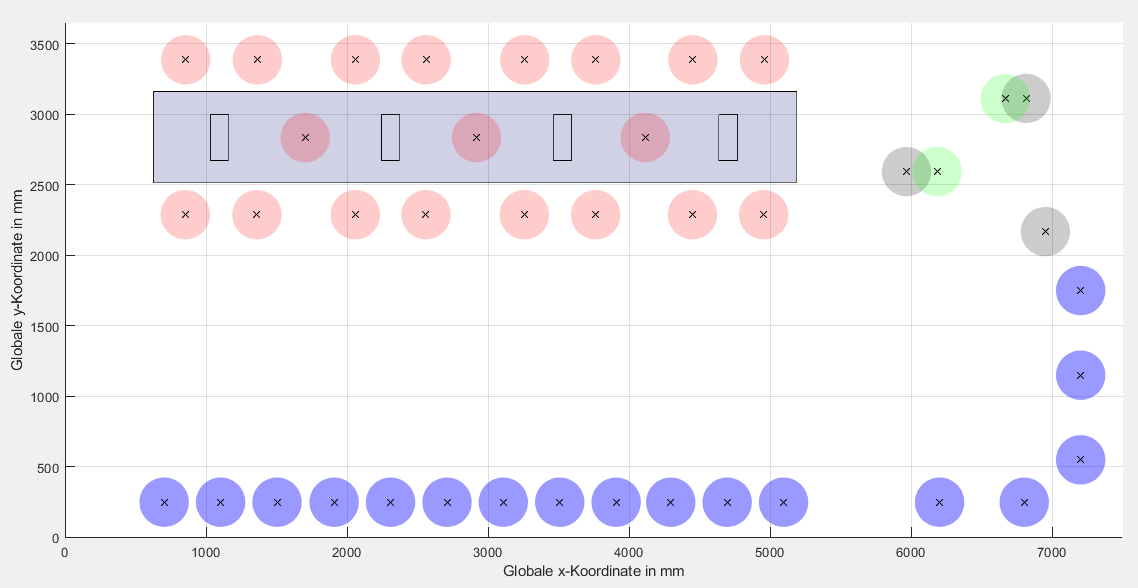
\includegraphics[width=0.8\textwidth]{grafiken/TransportbereichKarte.png}
	\caption{Bereichseinteilung}
	\label{fig:Bereiche}
\end{figure}